\documentclass{beamer}
\usepackage{diagbox}
\usepackage{tikz}
\usepackage{amsmath}
\usepackage{graphicx}
\usepackage[natbib=true,style=authoryear,backend=bibtex,useprefix=true]{biblatex}
\addbibresource{master_bibliography}
\usetikzlibrary{arrows.meta,positioning}
\usetikzlibrary{shapes.multipart,matrix,positioning,arrows,arrows.meta}
\usepackage[utf8]{inputenc}
\usefonttheme{serif}
% \usefonttheme{} % using non standard fonts for beamer
\usetheme{Hannover}

\AtBeginSection[]{
  \begin{frame}
  \vfill
  \centering
  \begin{beamercolorbox}[sep=8pt,center,shadow=true,rounded=true]{title}
    \usebeamerfont{title}\secname\par%
  \end{beamercolorbox}
  \vfill
  \end{frame}
}
%Information to be included in the title page:
\title[]{Coupled models of structured contagion processes in human-environment systems}
\author{Peter C. Jentsch}
\institute[]{Department of Applied Mathematics, University Of Waterloo}
\date{August 6th, 2021}
\begin{document}

\frame{
    \titlepage
    
\footnotesize
\centering{Supervised by Chris T. Bauch and Madhur Anand}
}

\setbeamerfont{frametitle}{size=\small}
\section{Introduction}
\begin{frame}{Contagious processes}
    \begin{itemize}
        \item A contagious process is one that is able to propagate itself through a set of hosts %(\citet{peterson1999contagious})
        \item Contagious processes shape our lives in many important ways
        \item Current situation has thrust the importance of modeling infections into popular consciousness 
    \end{itemize}
\end{frame}

\begin{frame}{Coupled systems}
    \begin{columns}
        \begin{column}[]{\textwidth}
            \begin{itemize}
                \item Coupling can often dramatically affect stability, e.g. coupled oscillators
                \item Human-environment systems focus on dynamics of humanity and the environment viewed as a whole
                \item This perspective provides useful answers to important problems
            \end{itemize}
        \end{column}
        % \begin{column}[]{0.3\textwidth}
        %     \begin{figure}
        %         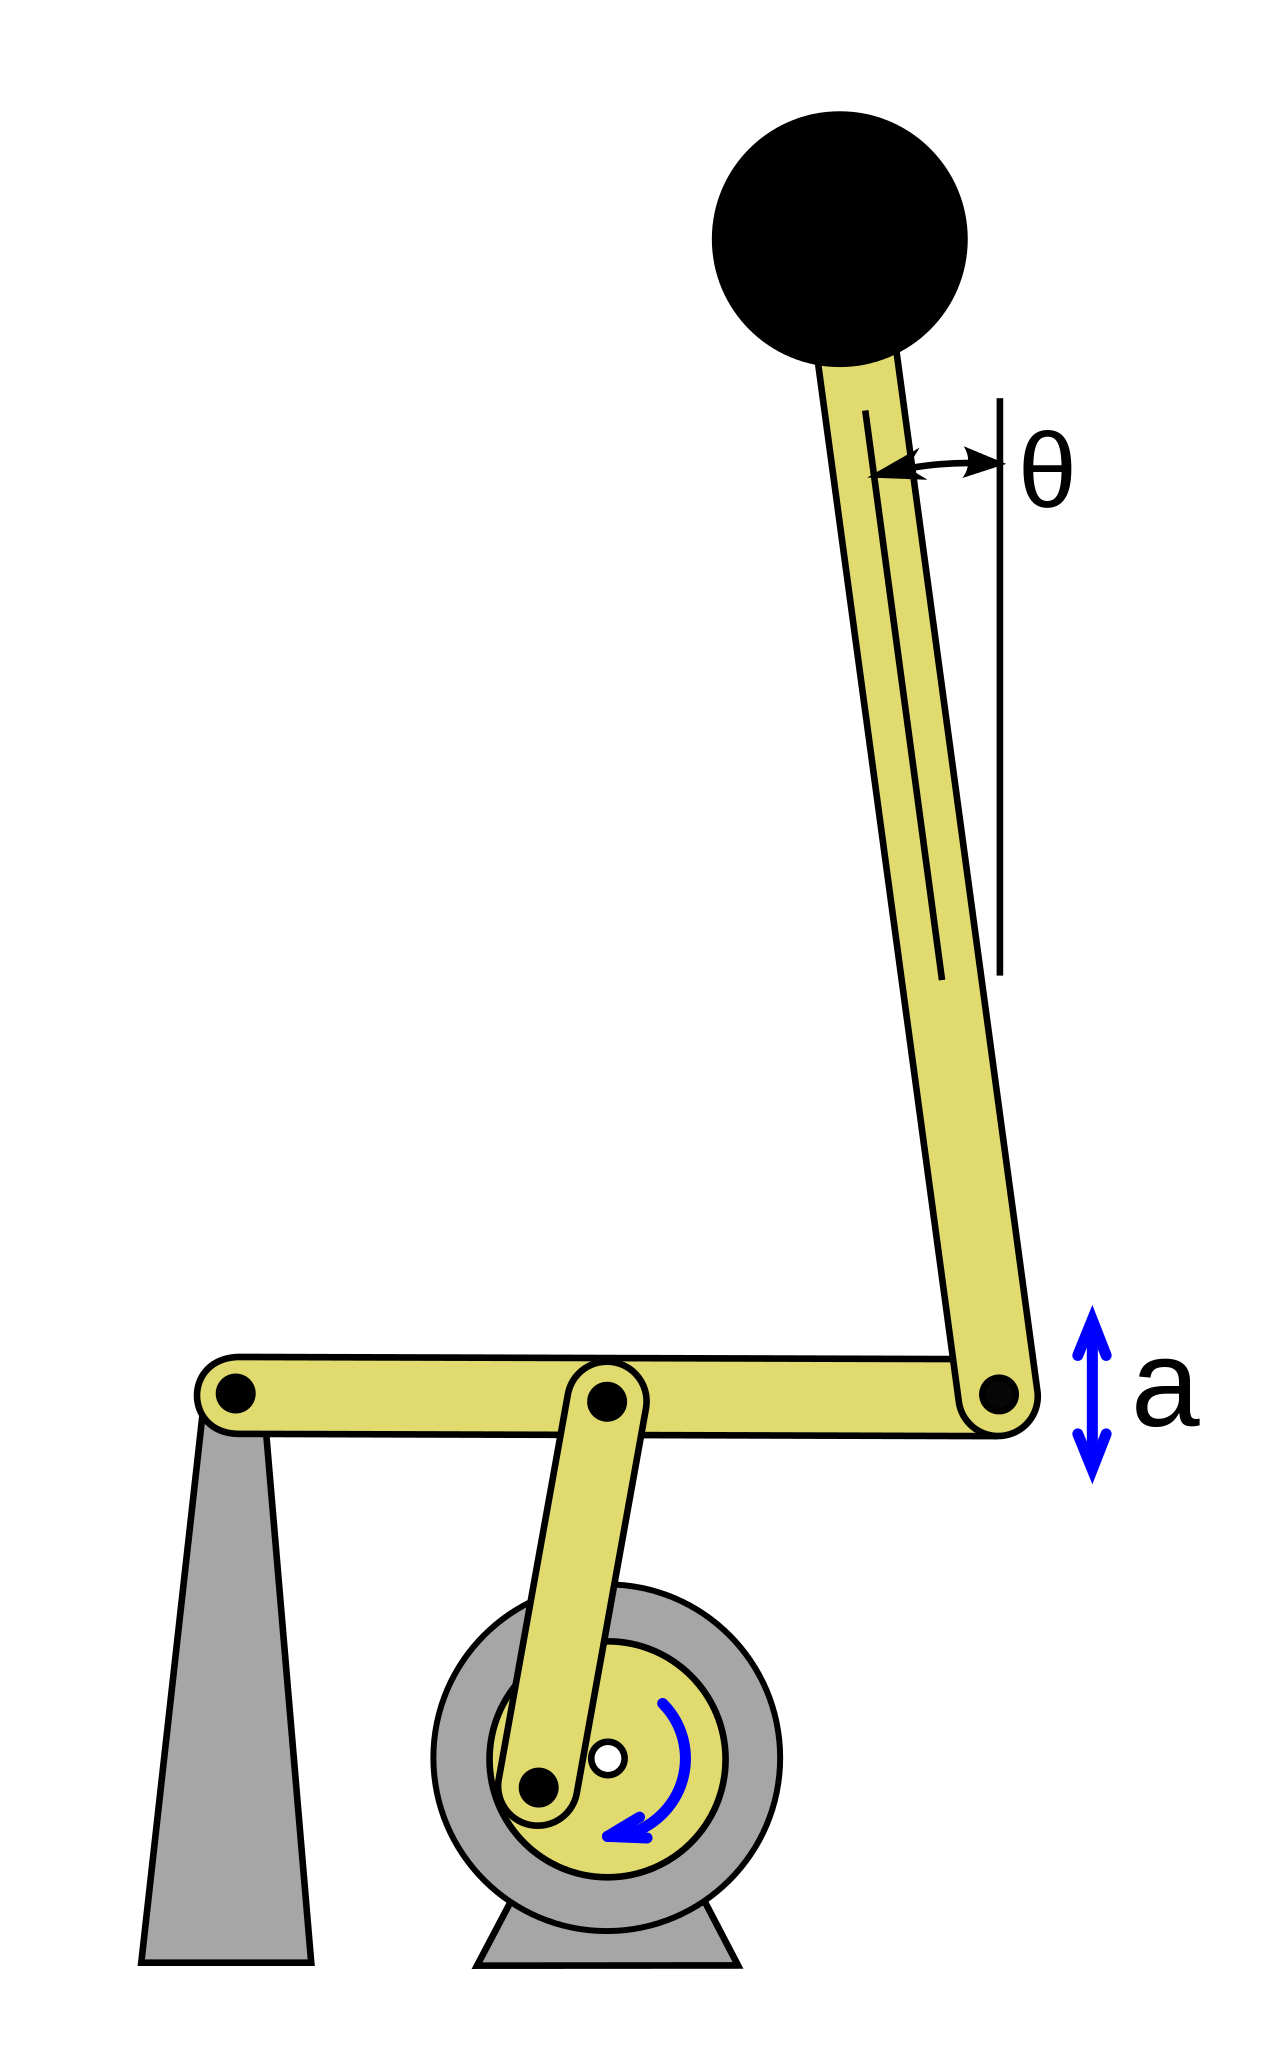
\includegraphics[width=\textwidth]{pendulum.png}
        %     \end{figure}
        % \end{column}
    \end{columns}
\end{frame}

\section{First Project}
\begin{frame}{Background}
    \begin{itemize}
        \item Population beliefs about the usage of non-pharmaceutical interventions (NPIs) can have a major effective on the epidemic landscape
        \item Population age distribution is a key factor in both NPI usage and COVID-19 mortality
        \item Vaccine rollout important to reducing mortality in the long term (\cite{bubar2020model,hoyt2020vaccine})
    \end{itemize}
\end{frame}
\begin{frame}

    Outline of project
    \begin{enumerate}
        \item Describe age-structured compartmental model of COVID-19 infection in a population, coupled to model of social distancing dynamics. 
        \item Fit model to data from Ontario, Canada
        \item Evaluate outcomes from different vaccination strategies, comparing vaccination of vulnerable populations vs vaccination of susceptible populations
    \end{enumerate}
\end{frame}
\begin{frame}{Compartmental model overview}
    \begin{columns}
        \begin{column}{0.4\textwidth}
        \scriptsize
        \textit{Disease Compartments}
            \begin{itemize}
                \item[$S_i(t)$] : Susceptible
                \item[$S_{2,i}(t)$] : Vaccinated but still susceptible
                \item[$V_i(t)$] : Vaccinated and immune 
                \item[$E_i(t)$] : Exposed 
                \item[$P_i(t)$] : Pre-symptomatic
                \item[$I_{a,i}(T)$] : Infectious and asymptomatic
                \item[$I_{s,i}(t)$] : Infectious and symptomatic
                \item[$R_i(t)$] : Recovered 
            \end{itemize}
        \tiny{where $i = 1 ... 16$} comprises age structure\\
        \footnotesize
        \vspace{0.1cm}
        \textit{Social compartments}
        \begin{itemize}
            \item[$x(t)$] : Uses NPIs
            \item[$1 - x(t)$] : Does not use NPIs
        \end{itemize}

        \end{column}

        \begin{column}{0.4\textwidth}
            \small


            \begin{figure}
                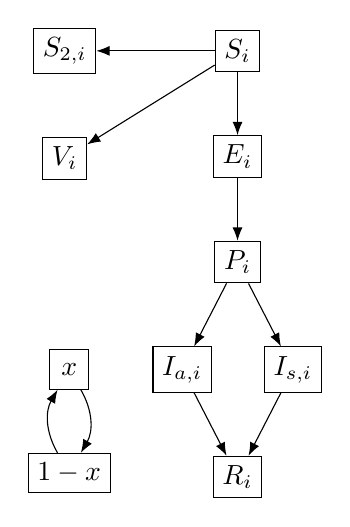
\begin{tikzpicture}[node distance=0.8cm, auto,
                    >=Latex, 
                    every node/.append style={align=center},
                    int/.style={draw, minimum size=0.5cm}]
                
                   \node [int] (S)             {$S_i$};
                   \node [int, below=of S] (E) {$E_i$};
                   \node [int, below=of E] (P) {$P_i$};
                   \node [int, below=of P, xshift=-20pt] (I_a) {$I_{a,i}$};
                   \node [int, below=of P, xshift=20pt] (I_s) {$I_{s,i}$};;
                   \node [int, below=of I_a, xshift=20pt] (R) {$R_i$};
                   \node [int, left=of S , xshift=-20pt] (S_2) {$S_{2,i}$};
                   \node [int, below=of S_2,yshift =0pt] (V) {$V_i$};
                   \path[->] (S) edge node[align=center] {} (E); %$r \rho_i  s(t)\left[(1 - \epsilon_P x(t))(C^H + C^O) + C^W(t) + C^S(t)\right]$\\$(I_s + I_a + P) - \tau$
                   \path[->] (E) edge node {} (P); %$\sigma_0$
                   \path[->] (P) edge node {} (I_a); %$\eta \sigma_1$
                   \path[->] (P) edge node {} (I_s); %$(1 - \eta) \sigma_1$
                   \path[->] (I_a) edge node {} (R); %$\gamma_a$
                   \path[->] (I_s) edge node {} (R); %$\gamma_s$
                   
                   \path[->] (S) edge node {} (S_2); %$v_{T} \frac{S(t)}{N - V(t)}$
                   \path[->] (S) edge node {} (V); %$v_{T} \frac{S(t)}{N - V(t)}$

                   \node [int, left=of I_a] (dist)             {$x$};
                   \node [int, below=of dist] (nodist) {$1-x$};
                   \path[->] (dist) edge [bend left] node {} (nodist); %$\displaystyle (1 - x)\left(\sum_{i=1}^{16}\alpha_i(I_{a_i} + I_{s_i}) - c x \right)$
                   \path[->] (nodist) edge [bend left] node {} (dist);
                \end{tikzpicture}
                \caption{Compartments}
            \end{figure}

        \end{column}

    \end{columns}
\end{frame}


\begin{frame}{Game theory as a model of NPI adoption}
    \begin{table}
    \footnotesize
    \begin{tabular}{ |c|c| c| } \hline
        \diagbox[width = 7em, height = 2em]{P1}{P2} &use NPI& don't use NPI   \\ \hline
        use NPI & \diagbox[width = 13em, height = 8em]{low risk,\\ NPIs unpleasant}{low risk,\\ NPIs unpleasant} &  \diagbox[width = 13em, height = 8em]{med risk,\\ NPIs unpleasant} {med risk}\\ \hline 
        don't use NPI & \diagbox[width = 13em, height = 8em]{med risk}{med risk,\\ NPIs unpleasant} &  \diagbox[width = 13em, height = 8em]{high risk}{high risk}   \\ \hline
    \end{tabular}
    \caption{NPI adoption as a two-player game (between P1 and P2)}
\end{table}
\end{frame}

\begin{frame}{Vaccination strategies}
    \begin{columns}
        \begin{column}{0.5\textwidth}
            We compare four vaccination strategies
            \begin{itemize}
                \item $>60$ first
                \item $<20$ first
                \item Uniform
                \item Contact-based
            \end{itemize}
            with respect to reduction in cumulative mortality after 5 years.
        \end{column}
        \begin{column}{0.5\textwidth}
        \begin{figure}
            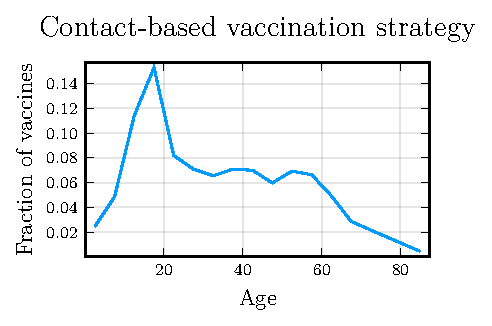
\includegraphics[width = \textwidth]{leading_eigenvector.pdf}
            \caption{\textbf{Vaccine allocation by age in the contact-based vaccination strategy}. Computed as the normalized leading eigenvector of the sum of the contact matrices.}
        \end{figure}
        \end{column}
    \end{columns}
\end{frame}
\begin{frame}{Parameterization}
    \begin{figure}
    \includegraphics[width=0.9\textwidth]{covid/plot_model.pdf}
    \caption{Model parameterization used, physical distancing matches reported cases.}
    \end{figure}
\end{frame}
\begin{frame}{Results}
            \begin{figure}
                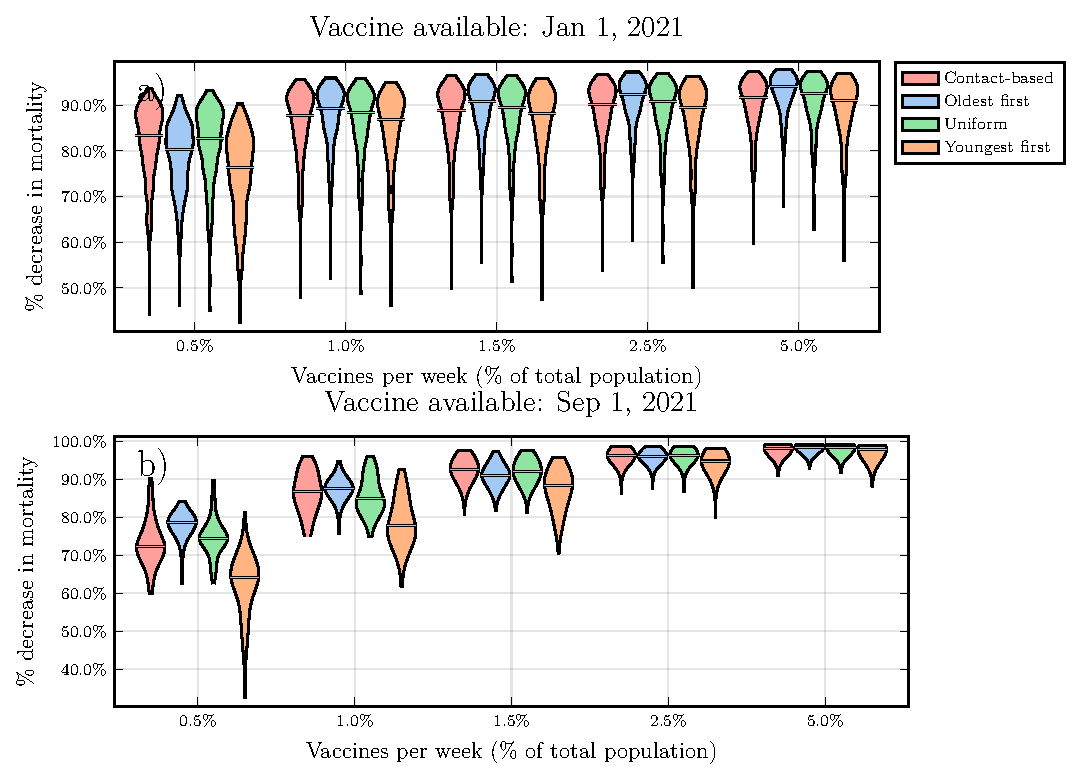
\includegraphics[width = 0.85\textwidth]{covid/vaccination_by_mortality_small.pdf}

                
                \caption{Percentage reduction in mortality for four strategies depends on vaccination start date and the vaccination rate.} %Percentage reduction in cumulative mortality due to COVID-19 after 5 years with respect to $\psi$, expressed as a percentage of the total population per week. Here $v_{D_i} = v_{T_i} = 0.75 $, shutdown at $200\%$ of first wave. Percentage reductions are relative to no vaccination. }
            \end{figure}
\end{frame}
\begin{frame}{}
    \begin{figure}
    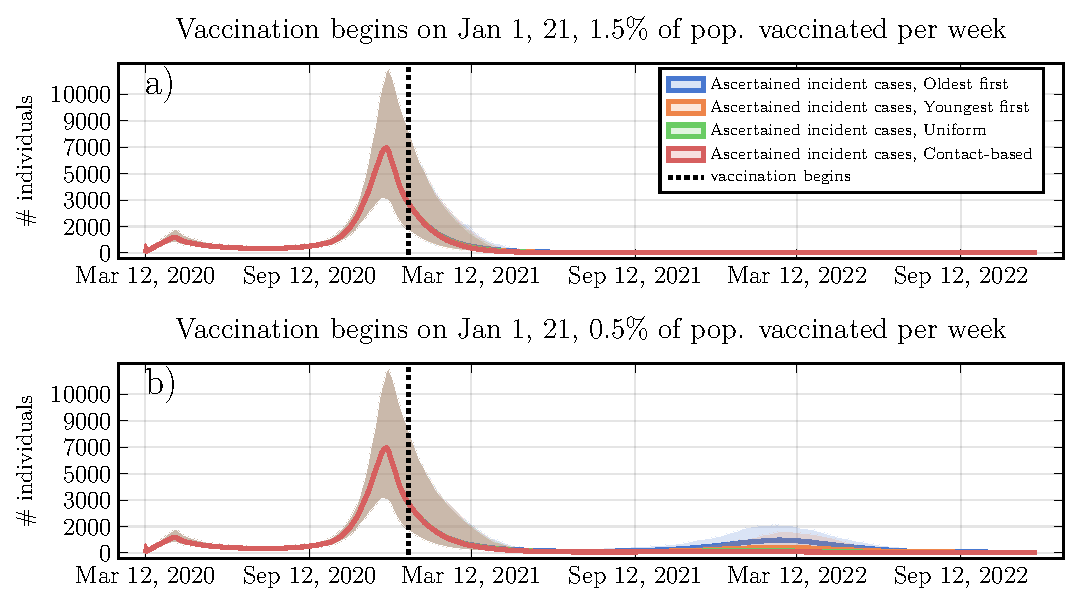
\includegraphics[width = \textwidth]{covid/main_text_ts_1.pdf}
    \caption{(a) timely vaccination prevents third wave, (b) partial vaccination and indirect protection help during the third wave}
    \end{figure}
\end{frame}
\begin{frame}{}
    \begin{figure}
    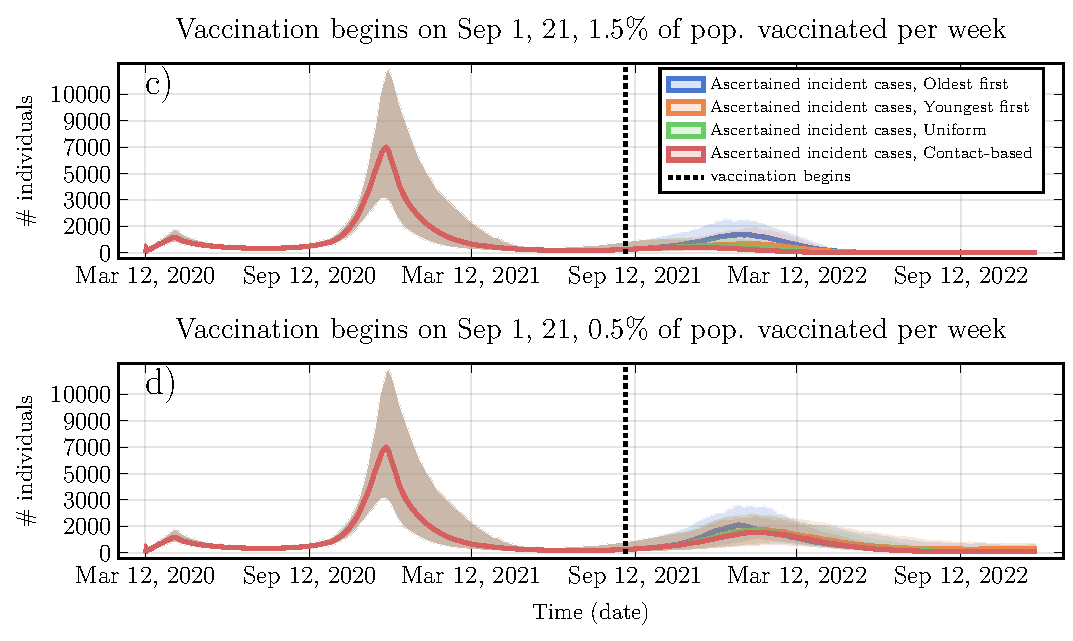
\includegraphics[width = \textwidth]{covid/main_text_ts_2.pdf}
    \caption{c) with a later start date but higher vaccination rate, partial vaccination and indirect protection help during the third wave as in b), (d) slow and late vaccination fails to prevent third wave.}
    \end{figure}
\end{frame}


\begin{frame}{Results}
    \begin{figure}
        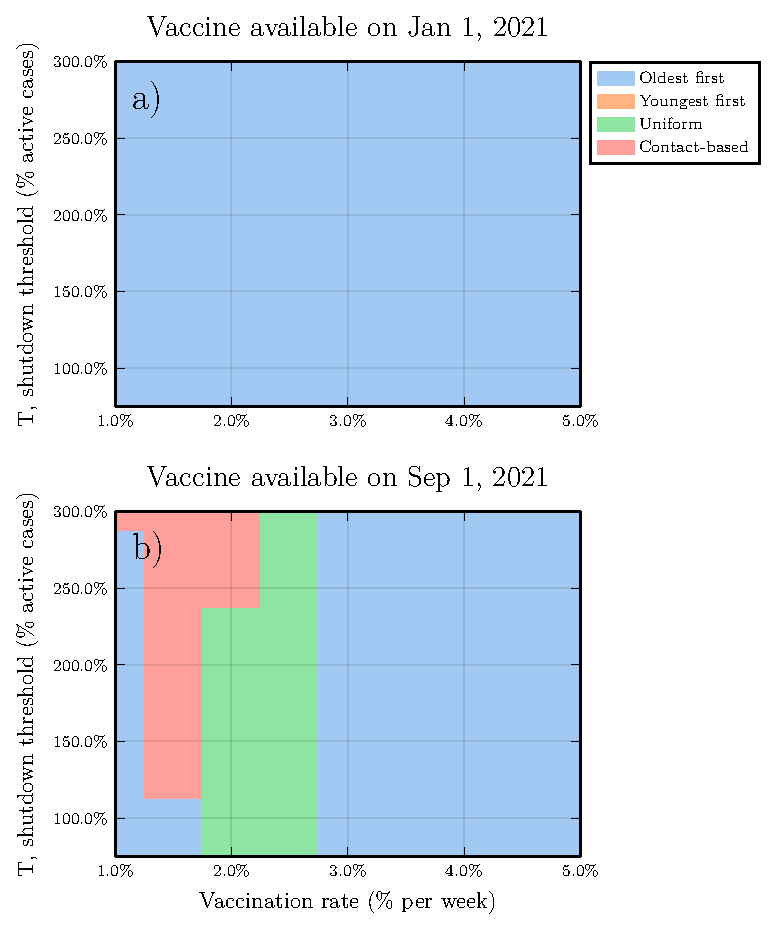
\includegraphics[height = 0.6\textheight]{covid/bivariate_heatmap.pdf}
        
        \caption{\small Later start to vaccination favours transmission-interrupting strategies for moderate vaccination rates. Each parameter pair is colored according to the strategy that prevents most deaths on average, over all realizations of the model.}
    \end{figure}
\end{frame}

\begin{frame}{Results}
\begin{figure}
    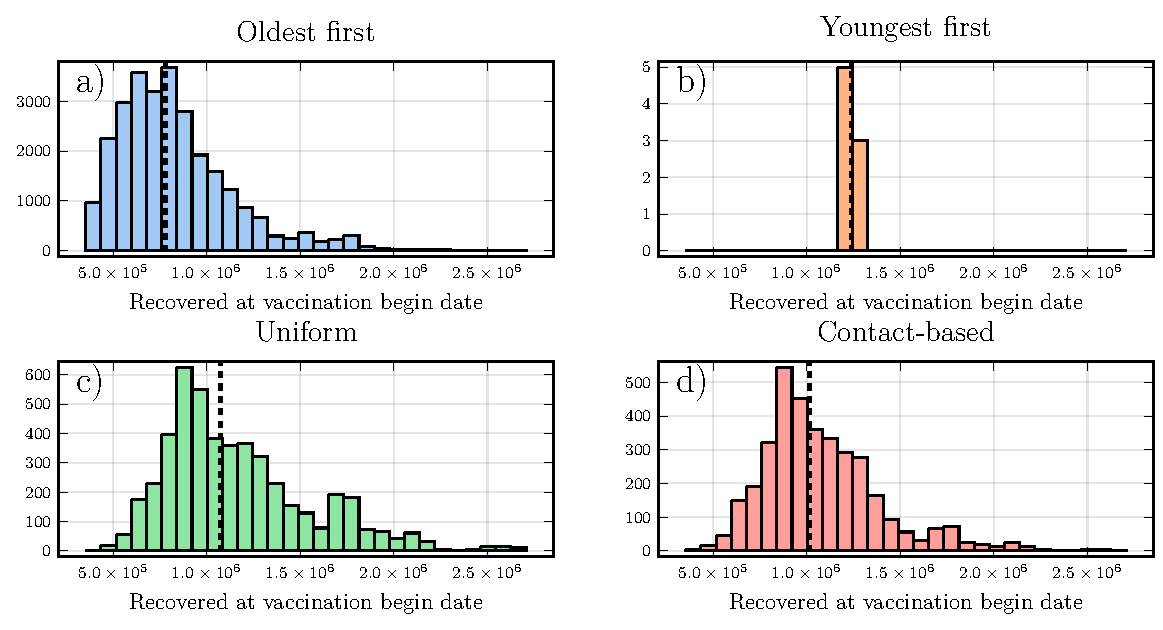
\includegraphics[width = \textwidth]{covid/histograms.pdf}
    \caption{\small More pre-existing natural immunity makes transmission-interrupting strategies more effective. Histogram of no. recovered at vaccination begin date, according to best strategy for that realization, over all parameter values in sensitivity analysis. Vertical lines are the median.}
\end{figure}
\end{frame}
\begin{frame}{Chapter Conclusion}
    \begin{itemize}
        \item We described an age structured compartmental model of Sars-CoV-2 infection and vaccination coupled to a social model 
        \item Showed that sometimes transmission interrupting strategies can be more effective
        \item Depends on the pre-existing immunity in the population
    \end{itemize}
\end{frame}





\section{Second Project}

\begin{frame}{Project 2}
    \begin{columns}
        \begin{column}{0.6\textwidth}
            \begin{itemize}
                \item Invasive forest pests cause incredible damage to ecosystems and lumber resources
                
                \item Evidence shows that movement of firewood is a major long distance vector (\citet{koch2014using})
                
                \item Education and awareness is a major way we try to reduce this vector
            \end{itemize}
        \end{column}
        \begin{column}{0.4\textwidth}
            \begin{figure}
                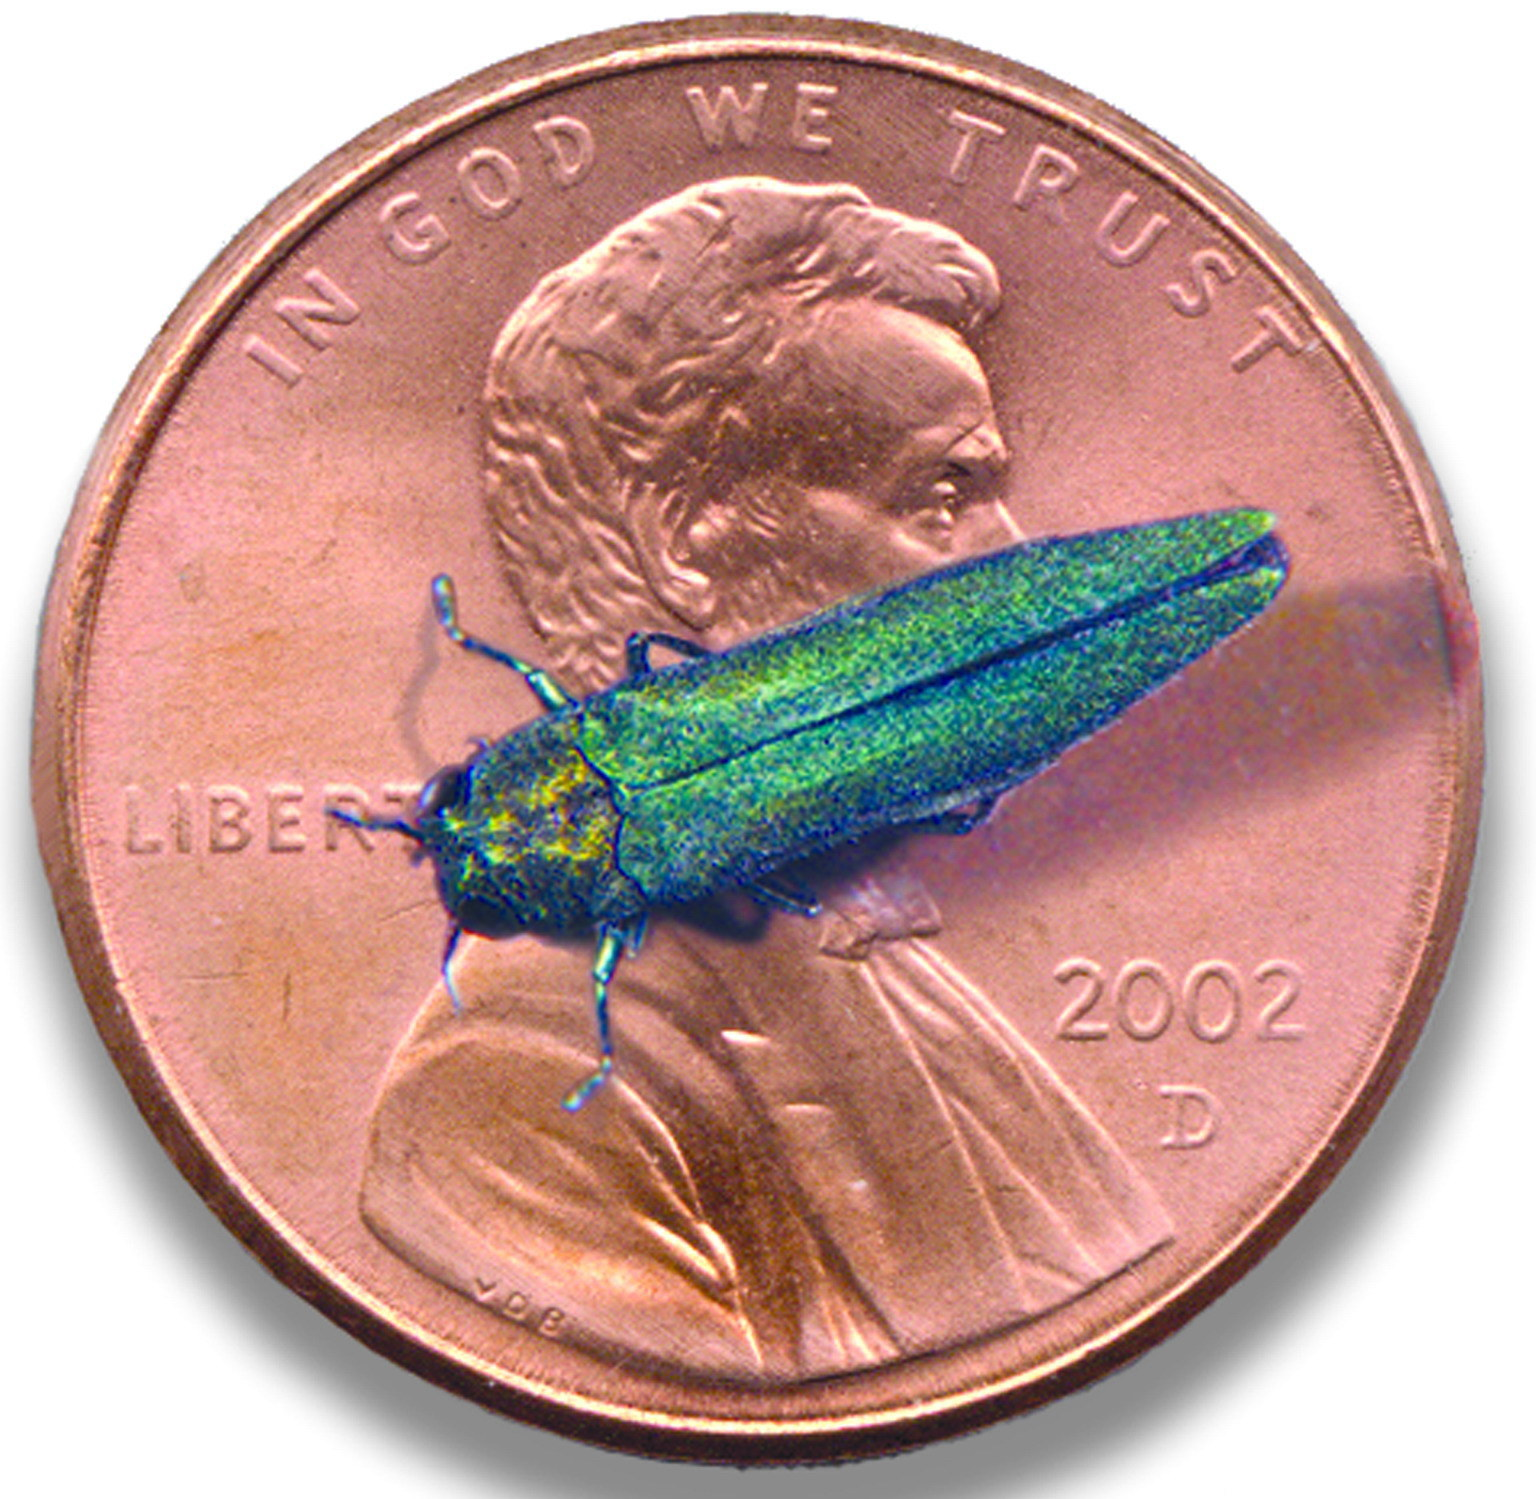
\includegraphics[width=\textwidth]{Emerald_ash_borer_penny.jpg}
                \caption{an Emerald Ash Borer, which devastated Ash populations in North America}                
            \end{figure}

        \end{column}
    \end{columns}
\end{frame}

\begin{frame}{Outline of project}
    \begin{enumerate}
    \item Adapt a model such as \citet{barlow2014modelling} to a larger, more realistic network
    \item Use model to compare three possible prevention measures
    \begin{itemize}
        \item Education/awareness
        \item Inspection of moved firewood
        \item Quarantine of highly susceptible forest patches
    \end{itemize}
    \item Assess measures across a range of parameter values and time horizons 
    \end{enumerate}
\end{frame}

\begin{frame}{Model}
    \footnotesize
    \begin{equation}
        \frac{d S_i}{dt} = \underbrace{ r S_i\left(1 - \frac{(S_i + I_i)}{K}\right)}_{\text{Logistic Growth Of Forest}} - \underbrace{A S_i (I_i+ B_i)\theta_k(I_i - I_a)}_{\text{Infestation term}}
        \protect \label{s_eqn}
        \end{equation}
        \begin{equation}
        \frac{d I_i}{dt} = \underbrace{-\gamma I_i}_{\substack{\text{Death of }\\\text{infested trees}}} + \underbrace{A S_i (I_i+ B_i)\theta_k(I_i - I_a)}_{\text{Susceptibles become infested}}- \underbrace{d\sum_{j = 1, j\neq i}^N P_{j,i} (1 - C_e) (1 - L_i)I_i}_{\substack{\text{Total infested wood }\\\text{leaving due to transport}}}
        \protect \label{i_eqn}
        \end{equation}
        \begin{equation}
        \frac{d B_i}{dt} = \underbrace{-\gamma B_i}_{\text{Decay of firewood}} + \underbrace{d\sum_{j = 1, j\neq i}^N P_{i,j} (1 - C_e) (1 - L_j)I_j}_{\text{Import of fallen wood}}
        \protect \label{b_eqn}
        \end{equation}
        \begin{equation}
        \frac{d L_i}{dt} = \sigma L_i (1 -L_i)(\underbrace{U}_{\substack{\text{Net cost to}\\\text{transport firewood}}} + \underbrace{s (2 L_i - 1)}_{\text{Social influence term}} + \underbrace{f I_i}_{\text{Impact of infestation}})  
        \protect \label{l_eqn}
    \end{equation}
        
\end{frame}

\begin{frame}{}    

    We use $T_i(t)$, computed from equation 5 to be the total number of infested trees in patch $i$ up to time $t$. 

    \begin{equation}
        \frac{dT_i}{dt}= A S_i (I_i+ B_i)\theta_k(I_i - I_a)
        \label{sum_eqn}
    \end{equation}

    Define $T(t) = \frac{1}{N} \sum_{i=1}^N T_i(t)$ to be the average total number of infested trees up to $t$.
\end{frame}


\begin{frame}{Data}

    \begin{figure}
        \includegraphics[width=0.7\textwidth]{firewood/core_graph_plot.png}
        \caption{Travel network used to weight edges in firewood transport network}
    \end{figure}
\end{frame}


\begin{frame}{Results}
    \begin{figure}
        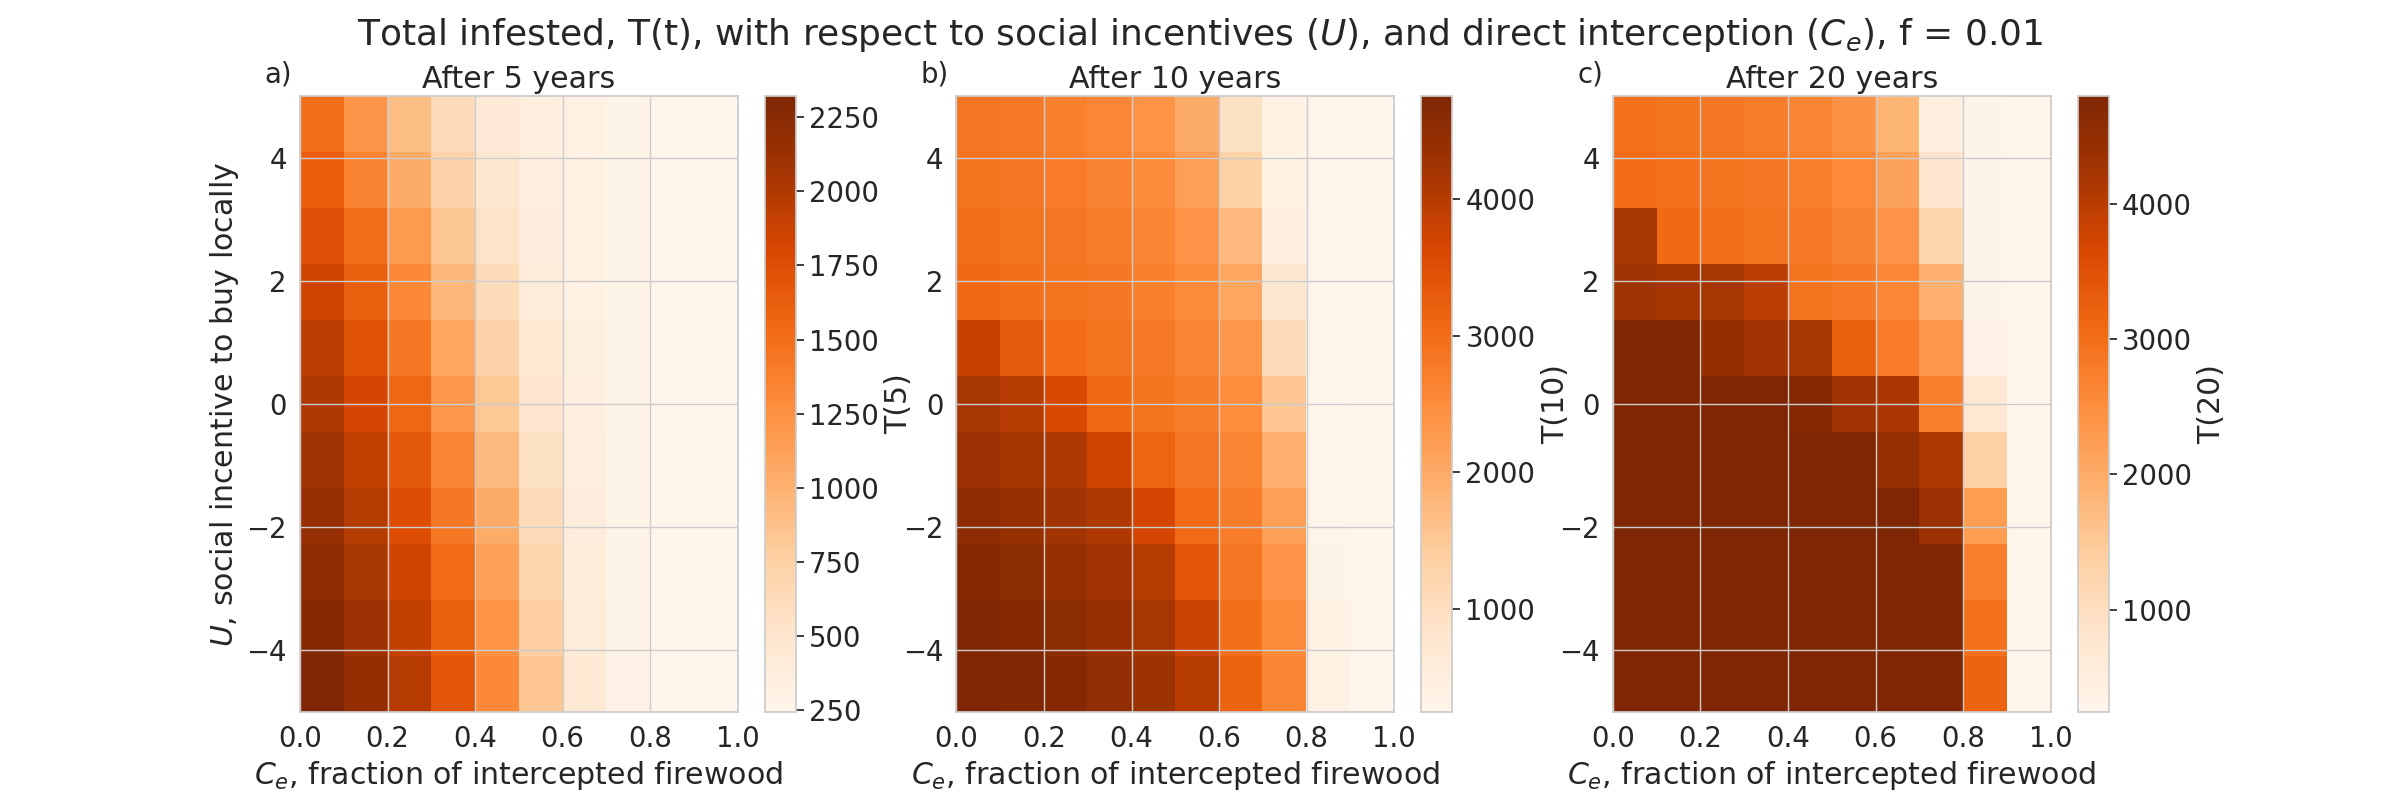
\includegraphics[width=\textwidth]{firewood/ct_v_ce_plane.png}
        \caption{Neither increasing $U$ nor $C_e$ are effective at long time scales. Total number of infested trees per node over 5 (a), 10 (b), and 20 (c) years}
    \end{figure}
\end{frame}

\begin{frame}{Results}
    \begin{figure}
        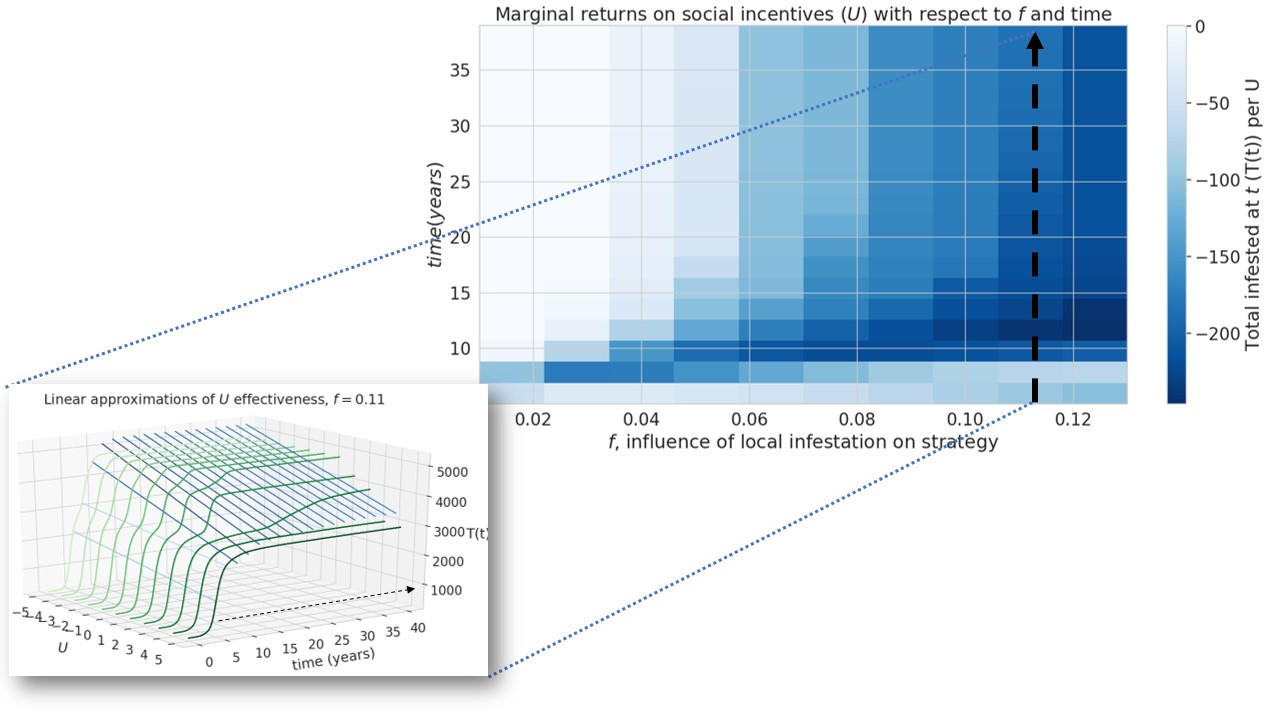
\includegraphics[width=\textwidth]{firewood/p1.jpg}
        \caption{\small The influence of infestation on transport strategy, $f$, can hinder the intervention by public outreach, in the long-term (after approximately 20 years). Efficacy of social incentives on infestation after time $T$. Inset graph shows an example of cross-section along the line $f = 0.11$}
    \end{figure}
\end{frame}

\begin{frame}{Results}
    \begin{figure}
        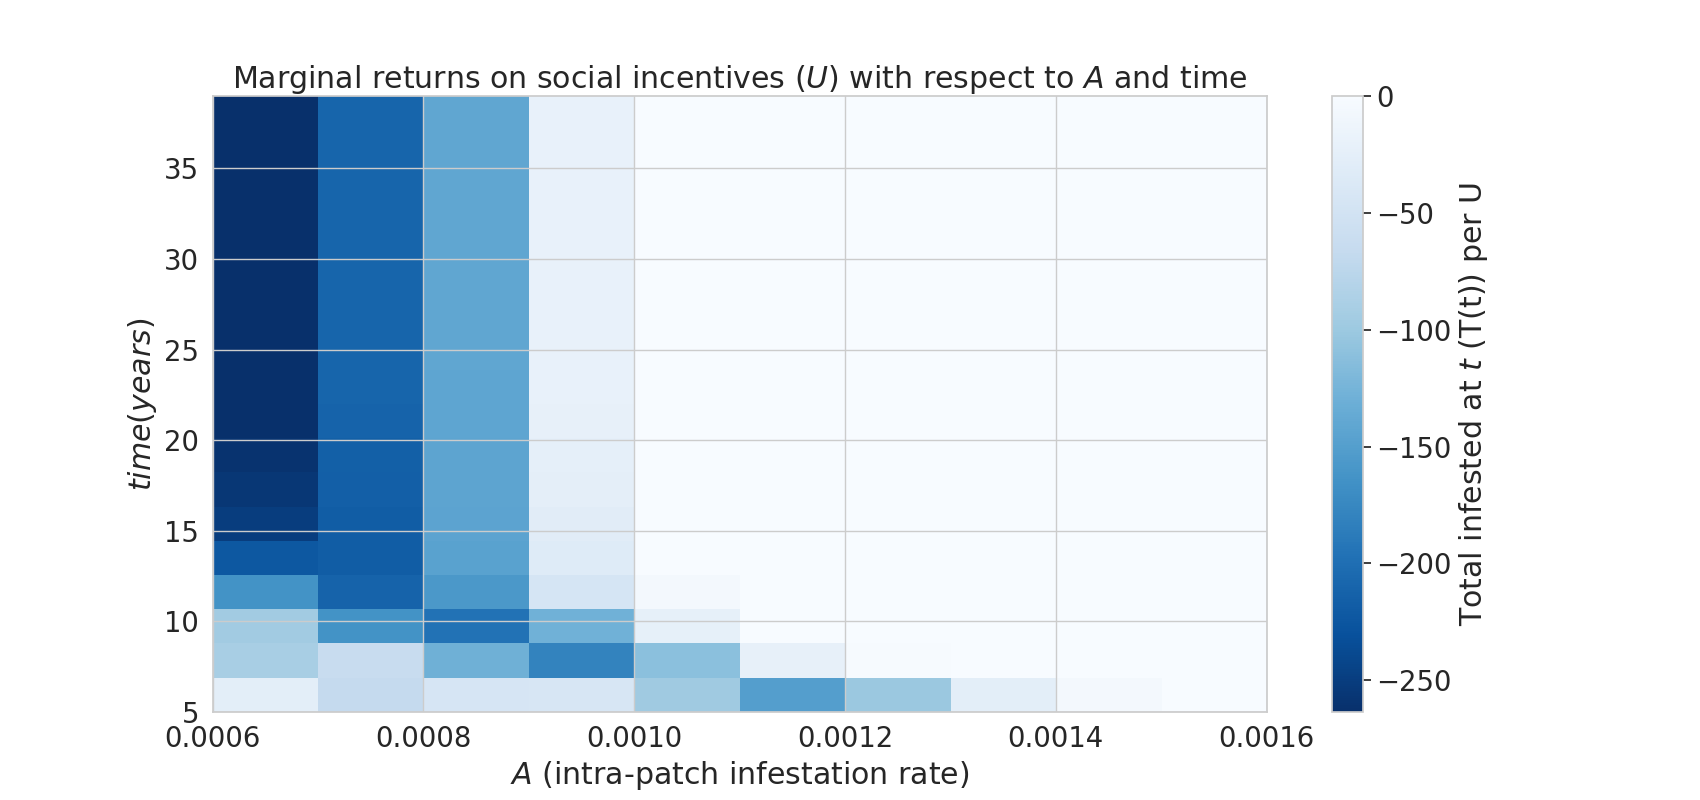
\includegraphics[width=\textwidth]{firewood/A_v_time.png}
        \caption{Increasing U becomes ineffective over time if $A$ is sufficiently large. Efficacy of social incentives on infestation after time period $T$ with respect to $A$, the intra-patch infestation parameter.}
    \end{figure}
\end{frame}

\begin{frame}{Results}
    \begin{figure}
        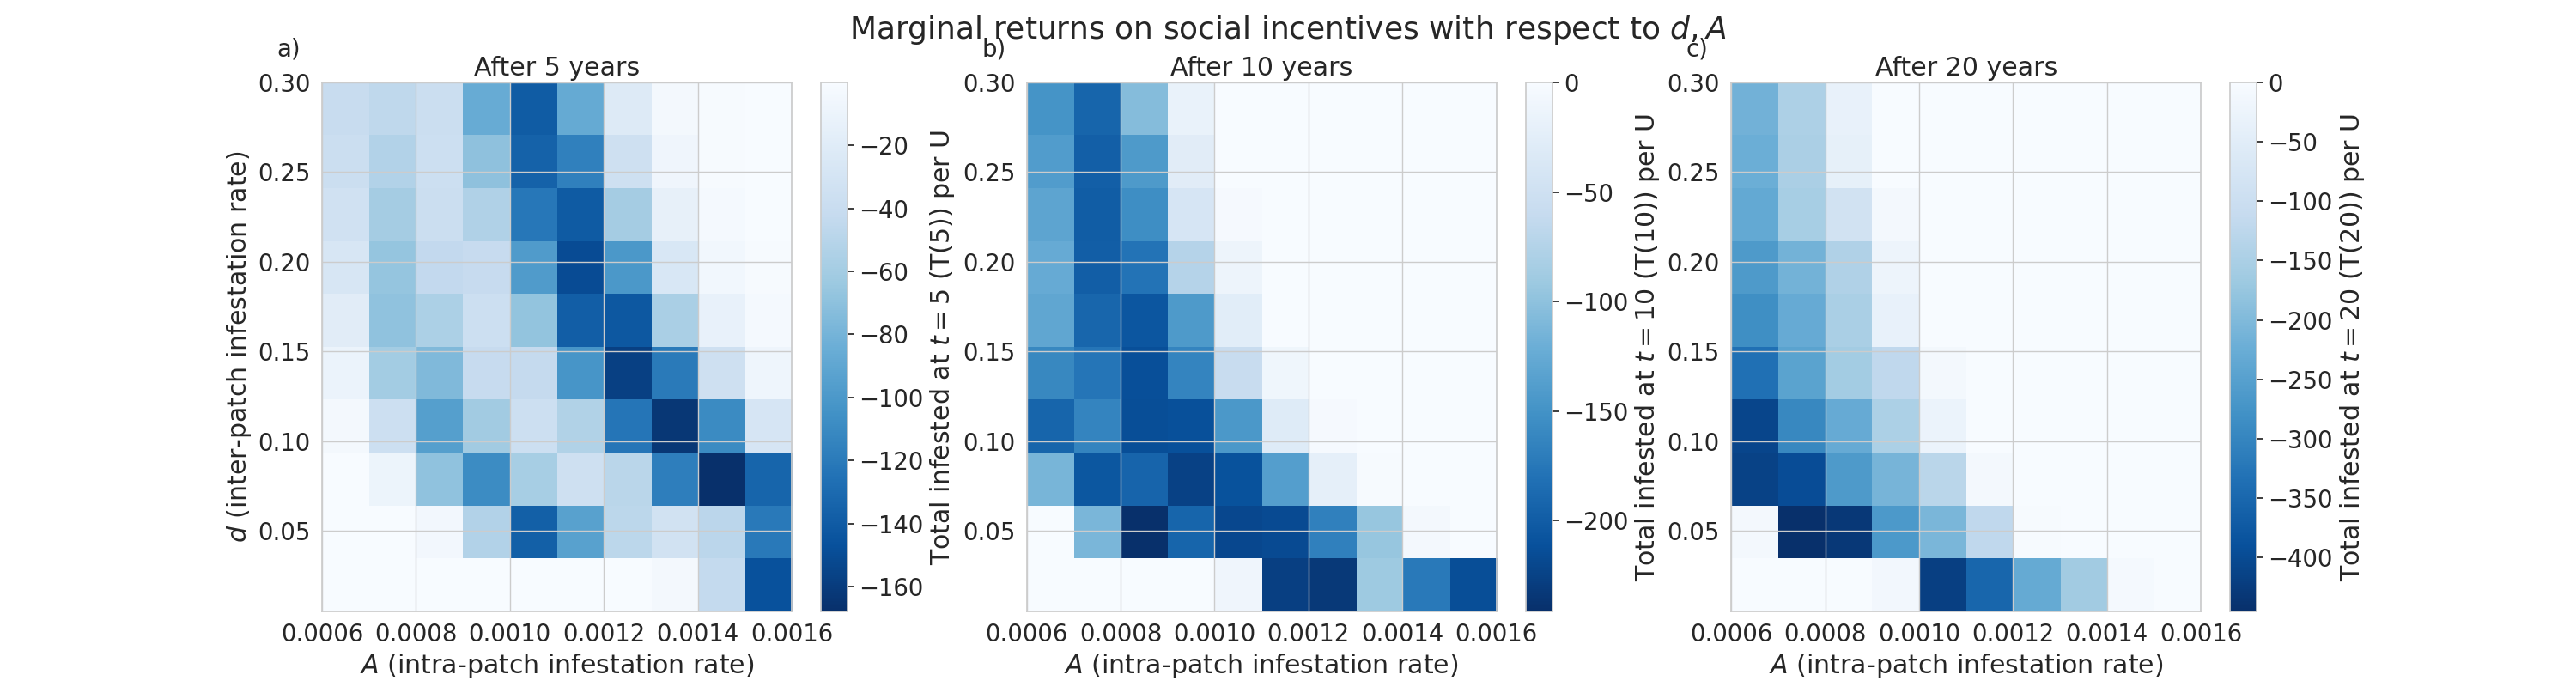
\includegraphics[width=\textwidth]{firewood/A_v_ct_v_d_marginal_gain.png}
        \caption{The social incentive to not transport firewood, $U$, is more effective with lower pest spread rates. Efficacy of social incentives on infestation after time $T$ intra-patch spreading rate $A$, affects infestation outcomes.}
    \end{figure}
\end{frame}
\begin{frame}{Results}
    \begin{figure}
        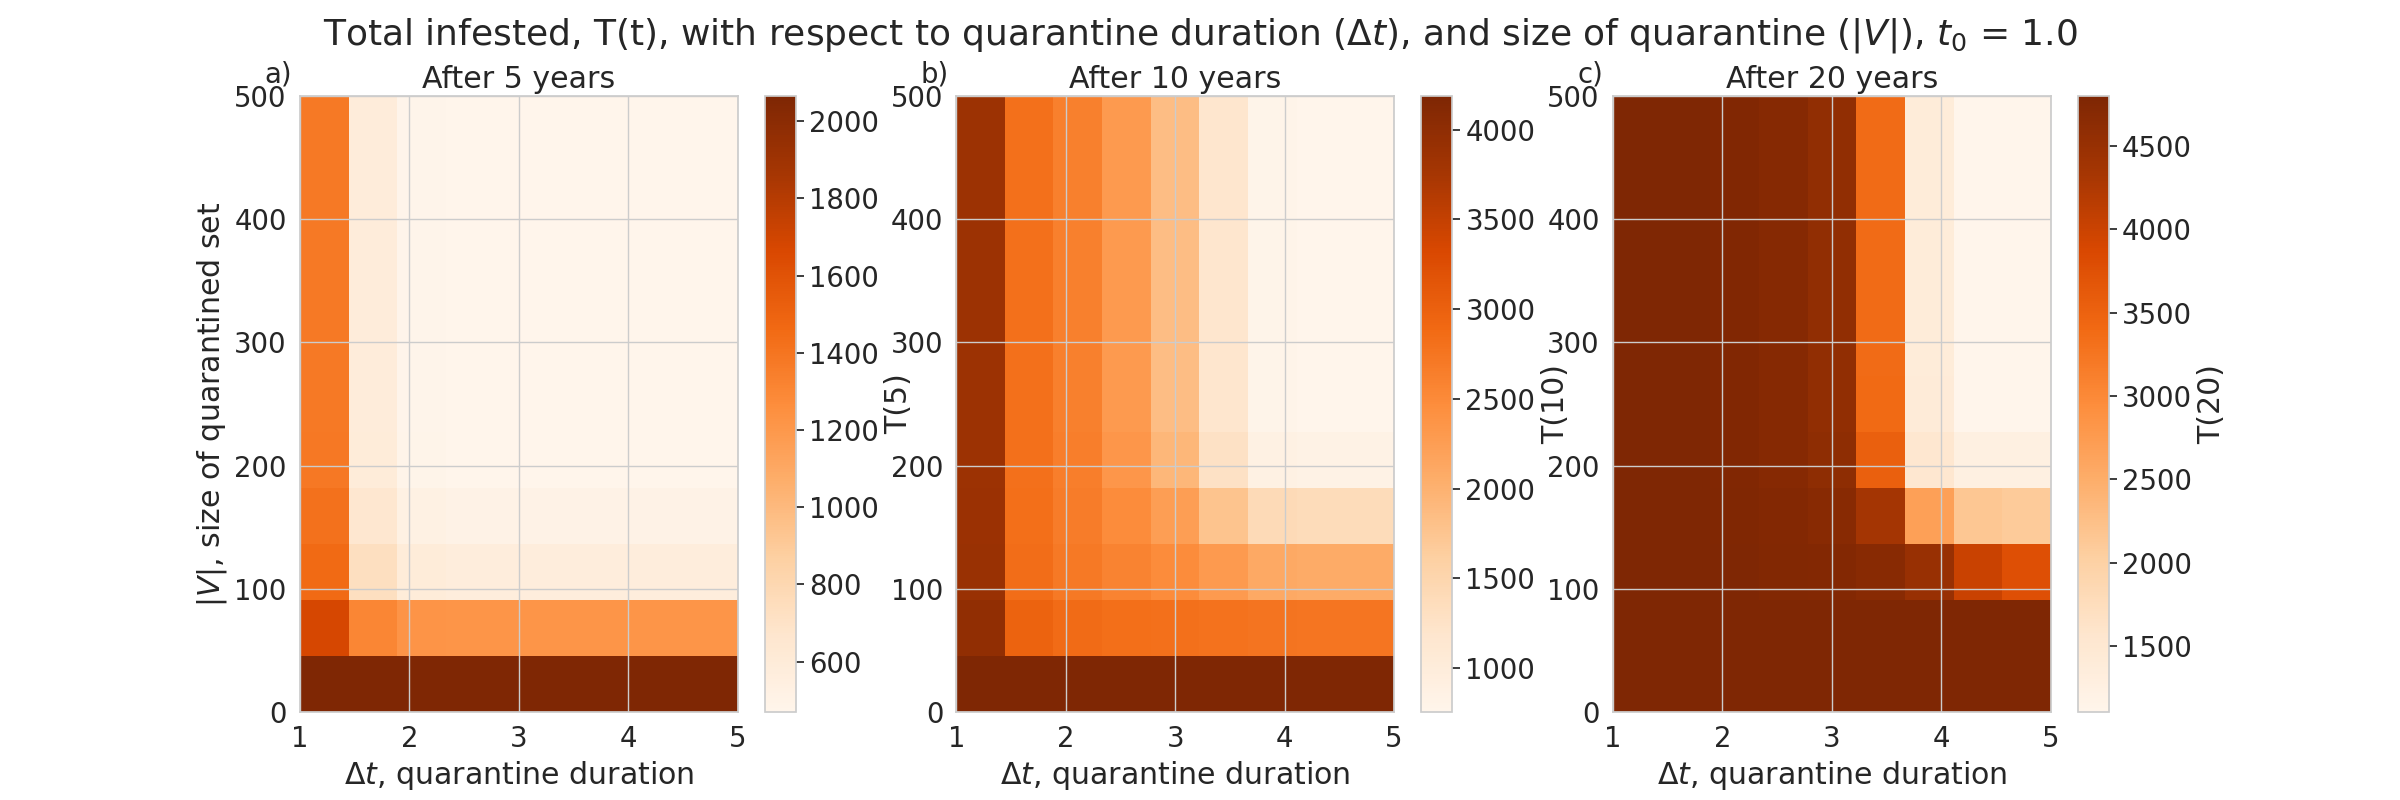
\includegraphics[width=\textwidth]{firewood/node_quarantine_plot_1.0.png}
        \caption{Quarantine needs to include many patches for long term effects. Average total infested trees ($T(t)$) after 5, 10 and 15 years (panels a), b), and c) respectively), assuming the quarantine begins one year after the pest is introduced.}
    \end{figure}
\end{frame}

\begin{frame}{Discussion}
    \begin{itemize}
        \item Firewood inspection not likely to be effective in implementation
        \item Education able to decrease infection in the short term, but dependent on pest-specific parameters
        \item Patch quarantine effective enough patches are isolated, and the pest is detected early 
    \end{itemize}
\end{frame}

\section{Third Project}
\begin{frame}{Background}
    \begin{itemize}
        \item Wildfire and bark beetles are disturbances integral to coniferous forest ecosystems in the western cordillera of North America (\cite{kaufmann2008status})
        \item Bark beetle outbreaks have always been destructive, but seem to be worse in recent decades
        \item Literature on causal relationship between bark beetle outbreaks and wildfire is extensive but inconclusive (\citet{axelson2009influence})
        \item Existing modelling of these two coupled disturbances is sparse
    \end{itemize}
\end{frame}

\begin{frame}{Project Outline}

    \begin{itemize}
        \item Extend existing model of \citet{duncan2015model} to include wildfires 
        \item Explore parameter regime of extended model
        \item Introduce forest stand thinning procedures to reduce MPB outbreaks
        \item Show that these stand thinning procedures are able to work due to increased stand heterogeneity 
    \end{itemize}
    
\end{frame}

\begin{frame}{Model}
    \begin{subequations}
        \footnotesize
        \begin{alignat}{2}
          j_{n+1, 1} &= d J_n + I_{n-2} + F_{n} \protect \label{eq1}\\
          j_{n+1, k} &= (1-d) j_{n, k - 1} - \frac{\alpha_1}{T} P_n j_{n,k-1  },\hspace{0.5cm} k = 2 ... K-1 ,K  \protect \label{eq2}\\
          S_{n+1} &= S_n + (1 - d) j_{n, K} - \left(I_n + \frac{\alpha_2}{T} P_n I_n\right) - \frac{\alpha_2}{T}P_n \left( S_n + (1-d) j_{n, K}\right) - \sigma_F \gamma_n  \protect \label{eq3}\\
          I_{n+1} &= r_1 I_n e^{-\beta_1 (T - S_{n+1})} - \frac{\alpha_2}{T} P_n I_n + \sigma_I \xi_n  \protect \label{eq4}\\
          F_{n+1} &=  P_n \left[\frac{\alpha_1}{T} \sum_{k = 1}^{K-1} j_{n,k} + \frac{\alpha_2}{T}\left( S_n + (1 - d)j_{n,K}\right) + \frac{\alpha_2}{T}I_n\right] + \sigma_F\gamma_n  \protect \label{eq5}\\
          P_{n} &= T - \sum_{i=1}^{n}  F_i e^{-\kappa (n - i)} \label{eq6}
        \end{alignat}
      \end{subequations}
\end{frame}

\begin{frame}{Results}
    \begin{figure}
        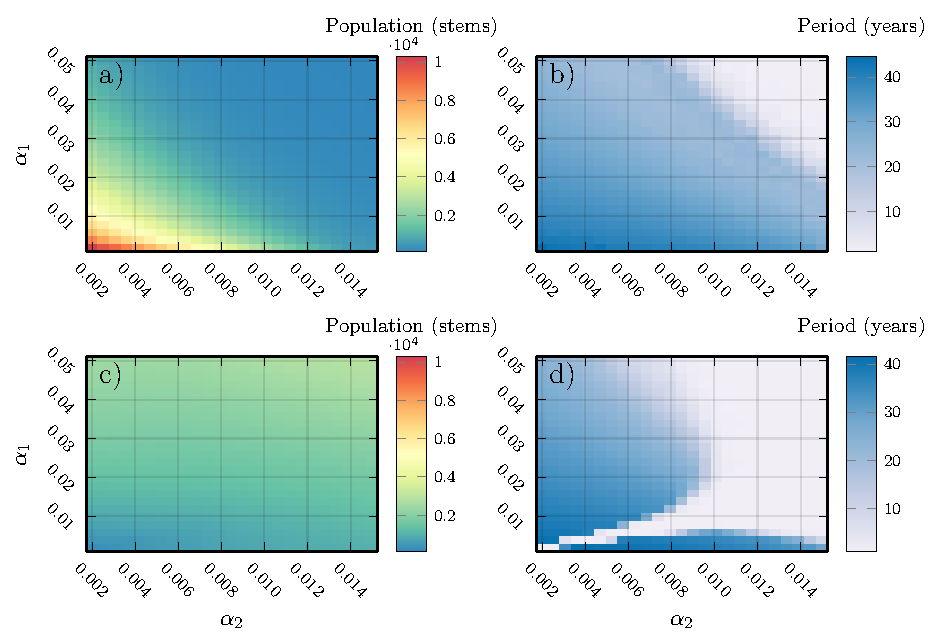
\includegraphics[width=0.7\textwidth]{mpb/a1_a2_phase.pdf}
        
        \caption{ \footnotesize Increasing burning rates $\alpha_1$,$\alpha_2$ reduce MPB outbreak size, cause stability in fire regimes. Panels: a) Average size of largest MPB population, b) Average frequency of MPB outbreaks, c) Average size of largest fire season, d) Average frequency of severe fire seasons. All measured at equilibrium. }
    \end{figure}
\end{frame}
\begin{frame}{Results}
    \begin{columns}
        \begin{column}[]{0.5\textwidth}
            \begin{figure}
                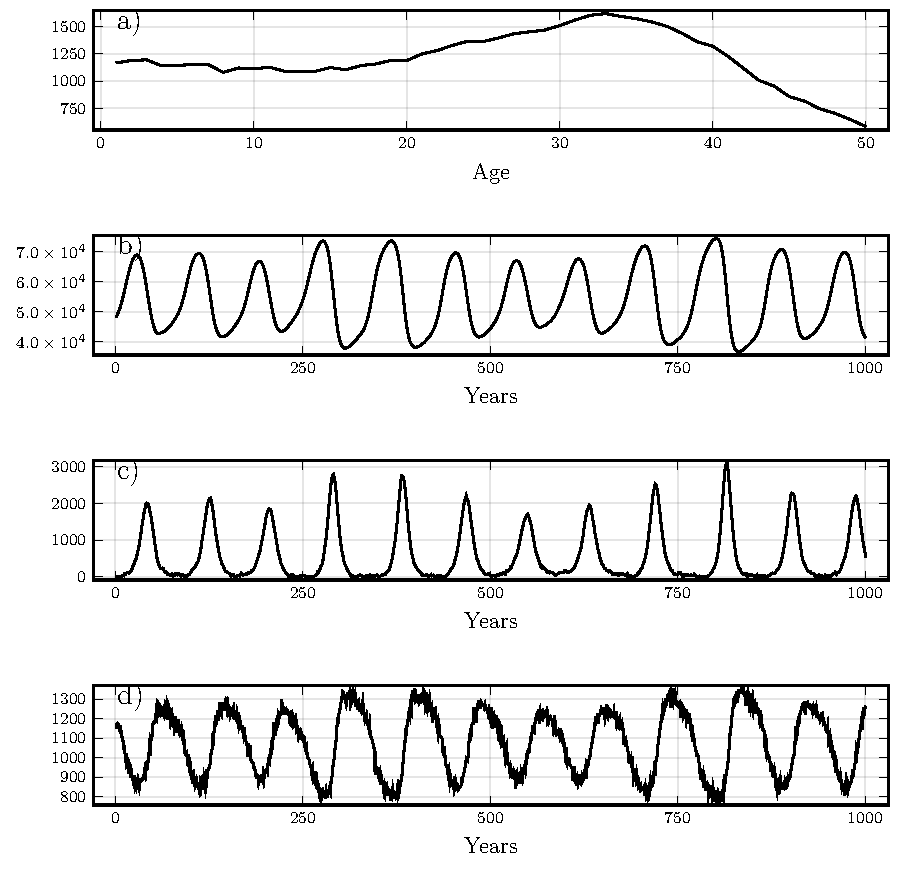
\includegraphics[width=\textwidth]{mpb/z1_ts.pdf}
                \caption{\small Without FTP, $\alpha_1 = 0.02,  \alpha_2 = 0.0025$, large even aged stands visible in juvenile age distribution (top panel).}
            \end{figure}
        \end{column}
        \begin{column}[]{0.5\textwidth}
            \begin{figure}
                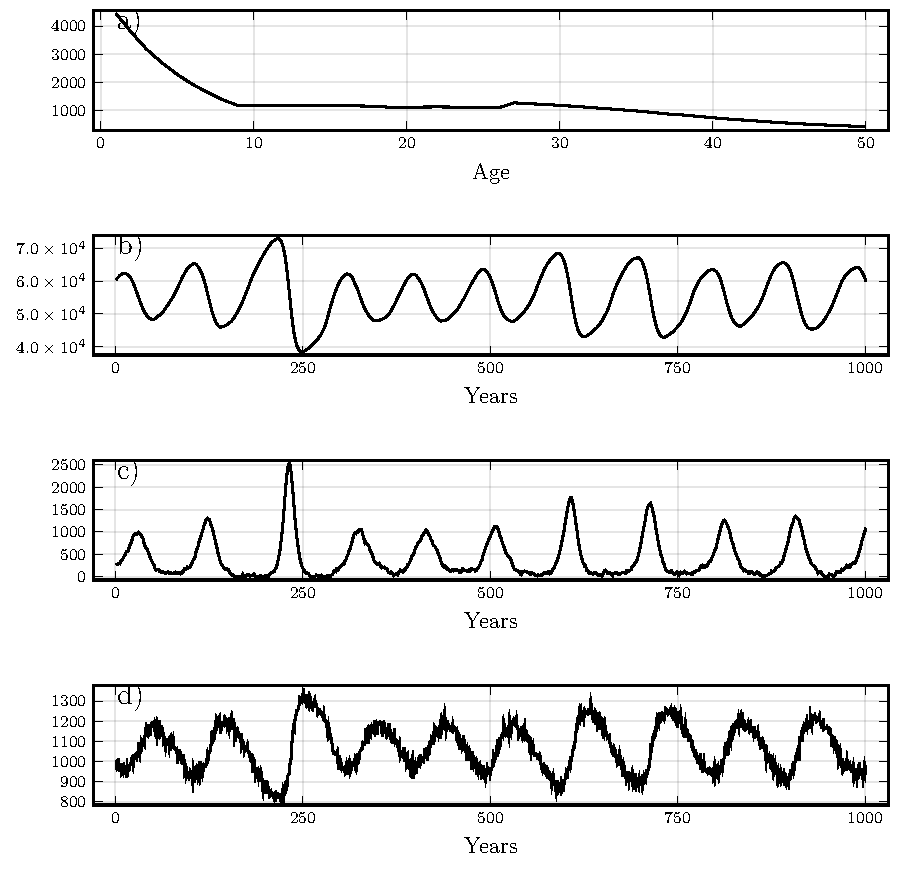
\includegraphics[width=\textwidth]{mpb/z1_ftp.pdf}
                \caption{\small With FTP, $\alpha_1 = 0.02, \alpha_2 = 0.0025$, $\tau = 0.15, m = 8$, with greater heterogeneity in juvenile age structure (top panel).}
            \end{figure}
        \end{column}
    \end{columns}
\end{frame}


\begin{frame}{Results}
    \begin{figure}
        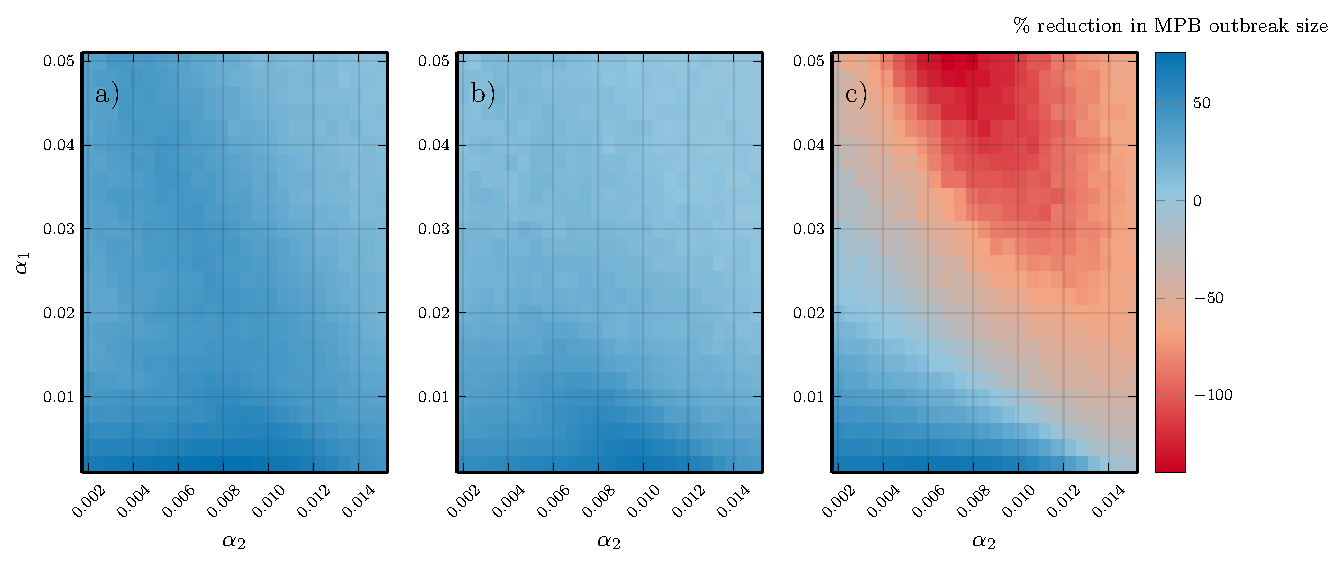
\includegraphics[width=\textwidth]{mpb/a1_a2_trim_gain.pdf}
        \caption{FTP most effective with small $\alpha_1$, CBP most effective with small $\alpha_1, \alpha_2$.  a) $\tau = 0.15, m = 8$, b) with $\tau = 0.15, m = 8$ applied every 5 years, c) controlled burning with $\tau = 0.15, m = 8$,  with respect to burning rates $\alpha_1,\alpha_2$.}
    \end{figure}
\end{frame} 

\begin{frame}{Chapter Conclusion}
    \begin{itemize}
        \item We show that increasing fire prevalence is able to dampen MPB outbreaks by increasing stand heterogeneity 
        \item Stand heterogeneity can also be increased through forest thinning or prescribed burning, which also dampens MPB outbreaks.
        \item These results are consistent with ecological evidence (\citet{seidl2016spatial,kaufmann2008status})
    \end{itemize}
\end{frame}


\begin{frame}{Overall conclusion}
\begin{itemize}
    \item Three models of coupled human-environment systems
    \item Compared methods of mitigation for respective coupled infectious processes
    \item Results obtained from these answer a gap identified in literature
\end{itemize}
\end{frame}


\begin{frame}{}
    \begin{center}
        \huge
        Thank you!
    \end{center}
\end{frame}

\begin{frame}[t,allowframebreaks]
    \printbibliography
\end{frame}


\end{document}


% \begin{frame}{Model Equations}

%     \tiny
%         \begin{eqnarray}
%             \frac{dS^1_i}{dt} &= & - r \rho_i s(t) S^1_i \sum_{j=1}^{16} C_{ij}(t) \left(\frac{I_{s_j} + I_{a_j} + P_j}{N_j}\right) - \tau S^1_i  \label{S1eqn} \\
%             \frac{dS^2_i}{dt} &= & - r \rho_i s(t) S^2_i \sum_{j=1}^{16} C_{ij}(t) \left(\frac{I_{s_j} + I_{a_j}+ P_j}{N_j}\right)  - \tau S^2_i  \label{S2eqn} \\
%             \frac{dE_i}{dt} &= &  r_i s(t) (S^1_i + S^2_i) \sum_{j=1}^{16} C_{ij}(t) \left(\frac{I_{s_j} + I_{a_j}+ P_j}{N_j}\right) - \sigma_0 E_i + \tau (S^1_i + S^2_i)\label{Eeqn} \\
%             \frac{dP_i}{dt} &= & \sigma_0 E_i - \sigma_1 P_i \label{Peqn} \\
%             \frac{dI_{a_i}}{dt} &= & \eta \sigma_1 P_i - \gamma_a I_{a_i}\label{Ieqn} \\
%             \frac{dI_{s_i}}{dt} &= & (1 - \eta) \sigma_1 P_i - \gamma_s I_{s_i} \label{Ieqn} \\
%             \frac{dR_i}{dt} &= & \gamma_a I_{a_i} + \gamma_s I_{s_i}  \label{Reqn} \\
%             \frac{dx}{dt} &= &\kappa x (1-x) \left(\frac{\sum_{i=1}^{16}\alpha_i(I_{a_i} + I_{s_i})}{\sum_{i=1}^{16} N_i} - c x\right) + p_{ul}(1-2 x)  \label{xeqn_new}\\
%     C_{ij}(t,x) &= & C^W_{ij}(t) + C^S_{ij}(t) + (1 - \epsilon_P x )\left({C}^O_{ij} + {C}^H_{ij}\right)
%         \end{eqnarray}
%     \end{frame}
% \begin{frame}{Studying COVID-19 vaccination}
%     \begin{itemize}
%         \item Model-based analyses are exploring which group should be the first to get the vaccine \cite{bubar2020model,hoyt2020vaccine}.
%         \item The epidemiological landscape will change throughout the remainder of the pandemic
%         \item Perception of risk due to the virus, and therefore perception of benefit of physical distancing, also fluctuates 
%         \item The group to vaccinate first, to most reduce mortality, is a function of this landscape
%         % \item Though many wealthy countries have already begun vaccination, many will not see significant doses of the vaccine for months/years, particularly in the global south \cite{mullard2020covid}
%     \end{itemize}
% \end{frame}

% \begin{frame}
% \frametitle{Social responses to the pandemic}
% \begin{columns}
%     \begin{column}{\textwidth}
%     \begin{itemize}
%         \item Non-pharmaceutical interventions (NPIs) can have a significant impact on SARS-CoV-2 transmission 
%         \item Pandemic waves are a creation of the population response to a pathogen
%         \item Important to model the incentive structures informing population response
%     \end{itemize}
%     \end{column}
% \end{columns}
% \end{frame}



% \begin{frame}{Incorporating age-structure}

%     \begin{itemize}
%         \item Age is an important factor in determining COVID-19 outcomes
%         \item Different age groups exhibit different contact patterns
%         \item Lockdowns affect age groups differently (work vs. school)
%         \item Each disease compartment is further divided into 16 age compartments
%         \item Interactions between age compartments defined by contact matrices
%     \end{itemize}

%     \begin{figure}
%         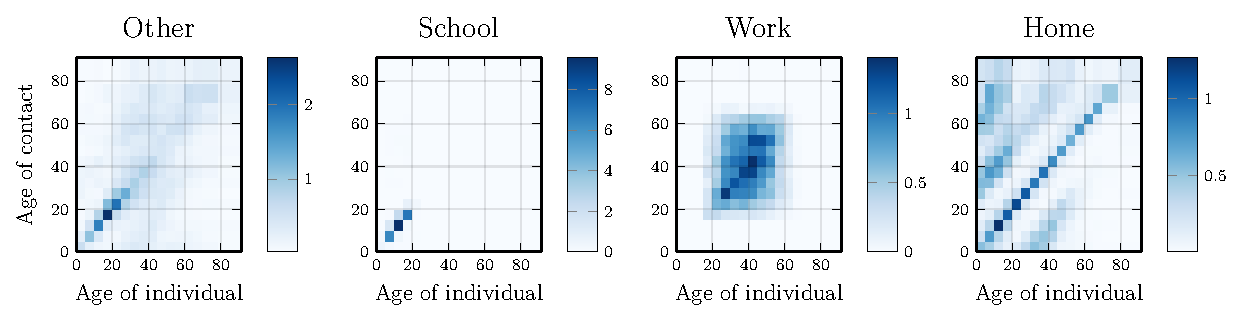
\includegraphics[width=\textwidth]{contact_matrices.pdf}
%         \caption{Contact matrices for Canada, mean contacts per day. Data from \cite{prem2017projecting}.}
%     \end{figure}
% \end{frame}


% \begin{frame}{Game theory as a model of NPI adoption}
%         \begin{table}
%         \footnotesize
%         \begin{tabular}{ |c|c| c| } \hline
%             \diagbox[width = 7em, height = 2em]{P1}{P2} &use NPI& don't use NPI   \\ \hline
%             use NPI & \diagbox[width = 13em, height = 8em]{low risk,\\ NPIs unpleasant}{low risk,\\ NPIs unpleasant} &  \diagbox[width = 13em, height = 8em]{med risk,\\ NPIs unpleasant} {med risk}\\ \hline 
%             don't use NPI & \diagbox[width = 13em, height = 8em]{med risk}{med risk,\\ NPIs unpleasant} &  \diagbox[width = 13em, height = 8em]{high risk}{high risk}   \\ \hline
%         \end{tabular}
%         \caption{NPI adoption as a two-player game (between P1 and P2)}
%     \end{table}
% \end{frame}
% \begin{frame}{Replicator equation for population games}
%         Population dynamics under a population game can be approximated by the replicator equation
%         \begin{equation}
%             \frac{d x}{d t} = \sigma x ( 1 - x)(-p(x,t))
%         \end{equation}
         
%         where

%         \begin{itemize}
%             \item $x(t)$ is the fraction of population using NPIs
%             \item $p(x,t)$ is the payoff function
%             \item $\sigma$ is the rate of population response
%         \end{itemize}
% \end{frame}

% \begin{frame}{Our model of NPI usage}

%     The full equation for $x(t)$, in this model, is given by

%     \begin{equation}{}
%         \frac{d x}{dt} = \sigma x (1 - x) \left(\frac{\sum_{i=1}^{16}\alpha_i(I_{a_i} + I_{s_i})}{\sum_{i=1}^{16} N_i} - c x\right) + p_{ul}(1-2 x) 
%     \end{equation}

%     \begin{itemize}

%     \item The term $p_{ul}(1-2 x)$ accounts for outside influence, where $p_{ul}$ is small.
    
%     \item $\alpha_i$ denotes the fraction of cases ascertained through testing.
    
%     \item $N_i$ is the population in age compartment $i$, $\sum_{i=1}^{16} N_i$ is the total population. 
%     \item $x(t)$ interacts with the infection dynamics by reducing the fraction of "home" and "other" contacts contributing to the infection rate
%     \end{itemize}

% \end{frame}


% \begin{frame}{Lockdown mechanics}
%     \begin{itemize}
%         \item There have been a few government-initiated lockdowns in Ontario, affecting schools and workplaces
        
%         \item Implemented in the model by reducing the contribution of the "work" and "school" contact matrices to the infection rate
        
%         \item Assume the government will initiate a partial or complete shutdown of workplaces and schools when the observed cases exceed some threshold $T$
%         \item We express $T$ as a percentage of the peak active cases during the first wave of the pandemic
%     \end{itemize}
    
% \end{frame}

% \begin{frame}{Vaccination mechanics}
%     \begin{itemize}
%         \item Implemented as an impulsive process, where we have $\psi$ vaccines available per day
%         \item The fraction of the $\psi$ people in age group $i$ that are immunized against severe disease is $\nu_{D_i}$
%         \item The fraction immunized against disease \emph{and} transmission is $\nu_{T_i}$
%         \item The allocation of vaccines to each age group $i$ is referred to as the vaccination strategy
%         \item Leftover vaccines are allocated uniformly to remaining non-empty compartments.
%         \item We also assume that some vaccines are "wasted" on people who are already recovered or infected, by modifying the vaccination per compartment by $\frac{S_i(t)}{N_i - V_i}$.
%     \end{itemize}

% \end{frame}


% \begin{frame}{Parameterization}
%     \includegraphics[width=\textwidth]{plot_model.pdf}
% \end{frame}

% \begin{frame}{Results}
%     \begin{columns}
%         \begin{column}{0.5\textwidth}
%             We compare four vaccination strategies
%             \begin{itemize}
%                 \item $>60$ first
%                 \item $<20$ first
%                 \item Uniform
%                 \item Contact-based
%             \end{itemize}
%             with respect to reduction in cumulative mortality after 5 years.
%         \end{column}
%         \begin{column}{0.5\textwidth}
%         \begin{figure}
%             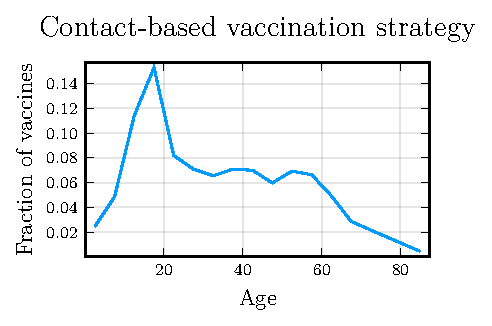
\includegraphics[width = \textwidth]{leading_eigenvector.pdf}
%             \caption{  The contact-based strategy is the normalized leading eigenvector of the sum of the contact matrices}
%         \end{figure}

      
%         \end{column}

%     \end{columns}


% \end{frame}